%!TEX options = -shell-escape

\documentclass[12pt]{report}
\usepackage[a4paper,twoside,top=20mm,bottom=20mm,inner=30mm,outer=25mm]{geometry}
\usepackage[utf8]{inputenc}
\usepackage[greek,english]{babel}
\usepackage[scaled=0.86]{couriers}
\usepackage[toc,page,title,titletoc]{appendix}
\usepackage[pdfpagelabels,unicode]{hyperref}
\usepackage{bookmark}
\usepackage[fixlanguage]{babelbib}
\selectbiblanguage{greek}
\usepackage{titlesec}
\usepackage{etoolbox}
\usepackage{graphicx}
\usepackage{array}
\usepackage{amsmath}
\usepackage{minted}
\usepackage{subcaption}
\captionsetup{compatibility=false}
\graphicspath{ {images/} }
\usepackage[noend]{algpseudocode}
\usepackage{algorithm}
\usepackage{afterpage}
\usepackage{comment}
\usepackage{longtable}

\newcommand\blankpage{%
    \null
    \thispagestyle{empty}%
    \addtocounter{page}{-1}%
    \newpage}

\hypersetup{
  colorlinks=true,
  % linkcolor=green,
  citecolor=red,
  % filecolor=blue,
  urlcolor=blue,
  % pdftitle=,
  % pdfauthor=,
  % pdfsubject=,
  % pdfkeywords=
}

\setcounter{secnumdepth}{3}
\setcounter{tocdepth}{3}

\titleformat{\chapter}
  {\normalfont\LARGE\bfseries}{\thechapter}{1em}{}
\titlespacing*{\chapter}{0pt}{3.5ex plus 1ex minus .2ex}{2.3ex plus .2ex}

\makeatletter
\patchcmd\@resets@pp{%
  \def\Hy@chapapp{\appendixname }%
}{%
  \def\Hy@chapapp{appendix}%
}{}{\errmessage{Cannot patch \string\@resets@pp}}
\patchcmd\@resets@ppsub{%
  \def\Hy@chapapp{\appendixname }%
}{%
  \def\Hy@chapapp{appendix}%
}{}{\errmessage{Cannot patch \string\@resets@pp}}
\makeatother

\addto{\captionsgreek}{\renewcommand{\appendixpagename}{Παραρτήματα}}
\addto{\captionsgreek}{\renewcommand{\appendixtocname}{Παραρτήματα}}
\addto{\captionsgreek}{\renewcommand{\appendixname}{Παράρτημα}}

\begin{document}
\selectlanguage{greek}

\hypersetup{pageanchor=false}

\begin{titlepage}
  \centering
  
\includegraphics[width=0.15\textwidth]{pyrforos}\par\vspace{1cm}
  {\scshape\LARGE Εθνικό Μετσόβιο Πολυτεχνείο\\
  Σχολή Ηλεκτρολόγων Μηχανικών και Μηχανικών Η/Υ\par}
  \vspace{1cm}
  {\scshape\Large Εργασία στο Μεταπτυχιακό Μάθημα\\
  Τεχνολογίες Λογισμικού Για Παροχή Υπηρεσιών σε Επικοινωνιακά Δίκτυα\par}
  \vspace{1.5cm}
  {\Large\bfseries Συστήματα Διαχείρισης Περιεχομένου Ανοιχτού Κώδικα\par}
  \vspace{2cm}
  {\large Δημήτριος Πολίτης (ΥΔ)\par}
  \vfill
  Επιβλέπων \par
  Καθ. Ευστάθιος Συκάς

  \vfill

% Bottom of the page
  {\large \today\par}
  \afterpage{\blankpage}
\end{titlepage}

\tableofcontents
\thispagestyle{empty}

\listoftables
\thispagestyle{empty}

\listoffigures
\thispagestyle{empty}

\begin{abstract}
Στο παρόν μελετώνται τα λογισμικά ανοιχτού κώδικα, τα οποία αφορούν σε διαχείριση περιεχομένου, με έμφαση στο \textlatin{web content} και τις δυναμικές ιστοσελίδες. Παρουσιάζονται αρχικά τα διαθέσιμα λογισμικά, τα πλεονεκτήματα και μειονεκτήματά τους και στη συνέχεια περιγράφεται αναλυτικά η διαδικασία δημιουργίας ενός ιστοτόπου \textlatin{Drupal} με τη χρήση αυτοματοποιημένων εργαλείων (\textlatin{ansible, vagrant}).

\vspace{10mm}

\noindent \textbf{Λέξεις κλειδιά:} Συστήματα Διαχείρισης Περιεχομένου, Ανοιχτός Κώδικας, Εξυπηρετητής Ιστοσελίδων Διαδίκτυο.
\end{abstract}

\hypersetup{pageanchor=true}
\clearpage
\pagenumbering{arabic}

\chapter{Εισαγωγή}\label{ch1}
\section{Εισαγωγή}
Στην εποχή του διαδικτύου λένε ότι υπάρχει κάποιος ή κάτι όταν έχει ηλεκτρονική παρουσία σε αυτό. Μπορεί αυτό να ακούγεται εν μέρει υπερβολικό, αλλά η εικόνα που παρουσιάζει μια εταιρία ή ένα φυσικό πρόσωπο στο διαδίκτυο επηρεάζει σε μεγάλο βαθμό την φήμη και την αξιοπιστία του.

Η δημιουργία, η συντήρηση και η ανανέωση του δυναμικού περιεχομένου των ιστοτόπων αποτελεί ένα δύσκολο αντικείμενια την διευκόλυνση του προσωπικού, το οποίο ασχολείται συστηματικά με τις παραπάνω εργασίες, έχουν αναπτυχθεί ειδικά εργαλεία, τα οποία ονομάζονται Συστήματα Διαχείρισης Περιεχομένου.

\section{Συστήματα Διαχείρισης Περιεχομένου}
Τα Συστήματα Διαχείρισης Περιεχομένου (\textlatin{Content Management Systems, CMS}) είναι εργαλεία δημιουργίας και διαχείρησης ιστοτόπων. Οι εφαρμογές αυτές εξαλείφουν την ανάγκη συγγραφής κώδικα προγραμματισμού~\cite{linode}. Από τη στιγμή την οποία έχουν αναπτυχθεί εντός των υποδομών, επιτρέπουν σε προσωπικό με μη εξειδικευμένες γνώσεις να διαχειρίζονται το περιεχόμενο των ιστοσελίδων τους.
Η επίπονη διαδικασία ανάπτυξης κώδικα για την ανανέωση των ιστοσελίδων, αντικαθίσταται από μια φιλική προς το χρήστη, διεπαφή.

\subsection{Πλεονεκτήματα}
Υπάρχουν αρκετές δεκάδες διαθέσιμα λογισμικά αυτού του είδους και πολλά από αυτά είναι δωρεάν - ανοιχτού κώδικα. Κάθε \textlatin{CMS} έχει διαφορετικά χαρακτηριστικά, δυνατότητες ή διεπαφή χρήστη. Οι εφαρμογές αυτές είναι διαθέσιμες σχεδόν από τα τέλη της δεκαετίας του 1990 και συνεχίζουν να χρησιμοποιούνται από όλο και περισσότερους χρήστες.

Πολλές φορές, ακόμα και έμπειροι προγραμματιστές προτιμούν την ευκολία ενός \textlatin{CMS} από το να γράψουν τον κώδικα για έναν ιστότοπο από την αρχή. Η χρήση των \textlatin{CMS} διευκολύνει την ταχύτερη ανάπτυξη του ιστοτόπου, εφόσον είναι αυτή δυνατή ακόμα και εντός λίγων ημερών. Παρέχει επίσης τη δυνατότητα παρακολούθησης των αλλαγών στον κώδικα με τη χρήση ενσωματωμένων εργαλείων \textlatin{version control}~\cite{wikipedia_2017:02}.

Όλο και περισσότερα \textlatin{CMS} είναι πλέον λογισμικά ανοιχτού κώδικα. Η ιδιότητά αυτή επιτρέπει στους χρήστες να αναπτύσσουν πρόσθετα (\textlatin{add-ons}) και να τεκμηριώνουν πληρέστερα τις λειτουργίες τους. Επίσης, είναι δυνατή η παροχή βοήθειας, ανταλλαγή απόψεων, σχολίων κτλ μεταξύ χρηστών.

Πολλά από τα \textlatin{CMS} δημιουργούν την δομή της ιστοσελίδας χρησιμοποιώντας θέματα. Τα θέματα βοηθούν στην καλή εμφάνιση της ιστοσελίδας, γεγονός το οποίο με τη σειρά του κάνει τους χρήστες να επιστρέφουν για νέο περιεχόμενο. Η αλλαγή θεμάτων και δομής της ιστοσελίδας είναι αρκετά εύκολη διαδικασία με τη χρήση \textlatin{CMS}. Επίσης πολλά από τα θέματα βασίζονται σε αρχεία \textlatin{CSS} ή \textlatin{HTML}, πράγμα το οποίο δίνει τη δυνατότητα στους προγραμματιστές να τα παραμετροποιούν σύμφωνα με τις ανάγκες τους και να διατηρούν μια σταθερή εμφάνιση σε όλες τις ιστοσελίδες. Τέλος, πολλά λογισμικά \textlatin{CMS} παρέχουν είτε δωρεάν επιπλέον θέματα, είτε επί πληρωμή, αυξάνοντας κατακόρυφα τις δυνατότητες των επιλογών.

Τα περισσότερα \textlatin{CMS} είναι φτιαγμένα ώστε να παρέχουν την απαραίτητη συμβατότητα με άλλα \textlatin{frameworks} ή \textlatin{standards}, αυξάνοντας την παραγωγικότητα και τις δυνατότητές τους~\cite{wikipedia_2017:02}.

Επίσης, τα \textlatin{CMS} έχουν τη δυνατότητα για αναβάθμιση όλων των λειτουργικών μερών τους με τη χρήση απλών οδηγών, φιλικών προς το χρήστη. Τις περισσότερες φορές παρέχεται και η δυνατότητα \textlatin{rollback}, εφόσον η διαδικασία δεν επιτευχθεί με επιτυχία.

Τα \textlatin{CMS} βοηθούν στην απλοποίηση των διαδικασιών και από την πλευρά των μη τεχνικών χρηστών, καθώς δεν απαιτούν κάποια εξειδικευμένη τεχνική γνώση για την ανάρτηση νέου περιεχομένου σε υπάρχουσες ιστοσελίδες, για παράδειγμα ιστολόγια.

Τέλος, τα \textlatin{CMS} παρέχουν ένα συγκεκριμένο επίπεδο ασφαλείας έναντι σε επιθέσεις εκμετάλευσης αδυναμιών στον κώδικα των ιστοσελίδων, καθώς πρόκειται για λογισμικά, τα οποία περνούν από εκτεταμένους ελέγχους κατά την ανάπτυξή τους, πριν την κυκλοφορία τους. Αυτό ισχύει τόσο για τα λογισμικά ανοιχτού κώδικα - τα οποία υποστηρίζονται συνήθως από μια μεγάλη κοινότητα χρηστών - όσο και τα εμπορικά \textlatin{CMS}. Στα παραπάνω αξίζει να προστεθεί το γεγονός ότι τα περισσότερα \textlatin{CMS} παρέχουν ενσωματωμένους μηχανισμούς παρακολούθησης και εξαγωγής συμπςερασμάτων από τα αρχεία καταγραφής.

\subsection{Μειονεκτήματα}
Τα λογισμικά \textlatin{CMS} έχουν ένα κύριο μειονέκτημα το οποίο κυρίως αφορά στον περιορισμό των δυνατοτήτων παραμετροποίησης μιας εφαρμογής, όταν αυτή αναμένεται να λειτουργήσει υπό διαφορετικά περιβάλλοντα. Για παράδειγμα, όταν μια εφαρμογή αναγκαστεί να λειτουργήσει πίσω από ένα πλήθος \textlatin{firewall} η \textlatin{reverse proxy}. Το παραπάνω πρόβλημα συνήθως αντιμετωπίζεται με \textlatin{plugins} στα πιο δημοφιλή \textlatin{CMS} (για παράδειγμα \textlatin{wordpress}).

Ένα ακόμα μειονέκτημα, το οποίο αφορά συνήθως στους διαχειριστές συστημάτων, είναι ότι τα περισσότερα \textlatin{CMS} απαιτούν ειδικές ρυθμίσεις - πολλές φορές μη-ασφαλείς ή εγκατάσταση ειδικών εργαλείων στους παραγωγικούς \textlatin{server} (για παράδειγμα \textlatin{drush - drushx} για το \textlatin{drupal}).

\section{Κατηγοριοποίηση των \textlatin{CMS}}
Τα \textlatin{CMS} μπορούν να κατηγοριοποιηθούν με βάση το περιεχόμενο, το οποίο πραγματεύονται, σε κατηγορίες όπως παρακάτω:

\paragraph{\textlatin{CMS} γενικής χρήσης} Τα \textlatin{CMS} αυτού του τύπου χρησιμοποιούνται για την κατασκευή ιστοσελίδων γενικού περιεχομένου. Συνήθως περιλαμβάνουν ενημερωτικό ή προωθητικό περιεχόμενο, χωρίς να περιλαμβάνουν αγοραπωλησίες. Τα τρία πιο διαδεδομένα σύγχρονα \textlatin{CMS} είναι λογισμικά ανοιχτού κώδικα, το καθένα με τα πλεονεκτήματα και τις αδυναμίες του.

\paragraph{\textlatin{CMS} ηλεκτρονικού εμπορίου} Συνήθως χρησιμοποιούνται για τη διαχείριση ηλεκτρονικών καταστημάτων. Αποτελούν στις περισσότερες των περιπτώσεων ολοκληρωμένα συστήματα διαχείρησης ηλεκτρονικών αγορών με λειτουργικότητες που εκτείνονται από την καταχώρηση της επιθυμίας ενός πελάτη στο καλάθι αγορών, μέχρι την εκδοσή τιμολογίων, αποστολή στον πελάτη, ακόμα και παρακολούθηση αποθεμάτων.

\paragraph{\textlatin{CMS} δημοπρασιών} Αποτελούν συναφή κατηγορία με την παραπάνω με τη διαφορά ότι αφορούν ηλεκτρονικές δημοπρασίες. Πολλές φορές μπορούν κάποια \textlatin{CMS} να ανήκουν και στις δυο κατηγορίες (π.χ. \textlatin{PHP-ProBid}).

\paragraph{\textlatin{CMS} διαχείρησης πολυμέσων (\textlatin{DAMS})} Αφορούν σε \textlatin{CMS} τα οποία χειρίζονται \textlatin{vlogs} ή σελίδες με πολυμέσα γενικότερα.

Στο παρόν παρουσιάζονται τα κυριότερα \textlatin{CMS} γενικού περιεχομένου, ανοιχτού κώδικα με έμφαση στα δημοφιλέστερα, με βάση το μερίδιο αγοράς του καθενός.

\chapter{Παρουσίαση των \textlatin{Open source CMS}}\label{ch2}
Παρακάτω παρουσιάζονται τα κυριότερα \textlatin{Open Source CMS} με μια συνοπτική περιγραφή και τα πλεονεκτήματα - μειονεκτήματά του. Επίσης για κάθε \textlatin{CMS} παρατίθεται και μια μικρή αποτύπωση του περιβάλλοντος αναρτήσης περιεχομένου.

\section{\textlatin{ExpressionEngine}}
Το \textlatin{ExpressionEngine} είναι ένα εμπορικό προϊόν το οποίο έχει στηθεί πάνω σε ένα \textlatin{opensource project}, Δίνοντας έτσι τα καλύτερα χαρακτηριστικά και από τους δυο τρόπους ανάπτυξης λογισμικού. Ως ένα εμπορικό λογισμικό το \textlatin{ExpressionEngine} υποστηρίζεται από μια ομάδα αφοσιωμένων \textlatin{developers} και εξειδικευμένων τεχνικών.
\begin{figure}[H]
\centering
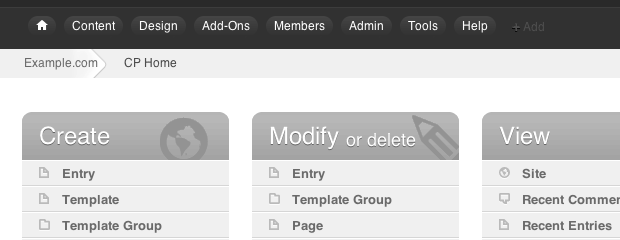
\includegraphics[width=0.9\textwidth, height=5cm]{ExpressionEngine-gray}
\caption{\textlatin{ExpressionEngine CMS}}
\label{fig:expr_eng}
\end{figure}

\section{\textlatin{Textpattern}}
Το \textlatin{Textpattern} είναι ένα κομψό \textlatin{CMS} το οποίο διατίθεται δωρεάν και είναι ανοιχτού κώδικα. Οι σχεδιαστές, οι \textlatin{developers} αλλά και οι \textlatin{blogers} μπορούν να βοηθηθούν από την ευελιξία και την επεκτασιμότητα του. Αποτελείται από μια εξελιγμένη μηχανή που μπορεί να χρησιμοποιηθεί για την υποστήριξη οποιουδήποτε τύπου ιστοσελίδας απαιτηθεί.
\begin{figure}[H]
\centering
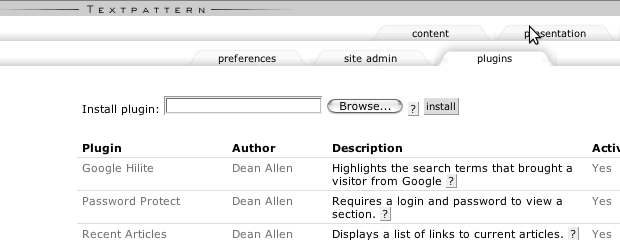
\includegraphics[width=0.9\textwidth, height=5cm]{Textpattern-gray}
\caption{\textlatin{Textpattern CMS}}
\label{fig:text_patrn}
\end{figure}

\section{\textlatin{Symphony CMS}}
Το \textlatin{Symphony} είναι ένα \textlatin{content management system (CMS)} το οποίο δίνει τη δυνατότητα στους χρήστες να δημιουργούν και να διαχειρίζονται ιστοσελίδες και \textlatin{web applications} ανεξαρτήτως μεγέθους – από τα απλούστερα \textlatin{blogs} εώς και τις πιο περίπλοκες ιστοσλίδες ειδήσεων ή κοινωνικών δικτύων.
\begin{figure}[H]
\centering
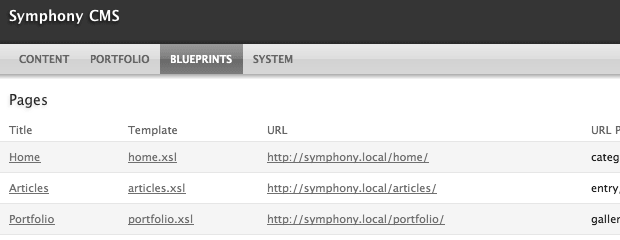
\includegraphics[width=0.9\textwidth, height=5cm]{symphony_cms-gray}
\caption{\textlatin{Symphony CMS}}
\label{fig:symphony_cms}
\end{figure}

\section{\textlatin{CMS Made Simple}}
Το \textlatin{CMS Made Simple™} είναι ένα λογισμικό ανοικτού κώδικα, το οποίο διανεμήθηκε στην πρώτη του έκδοση τον Ιούλιο του 2004. Στηρίζεται στην γλώσσα \textlatin{PHP} και παρέχει στους \textlatin{developers} έναν απλό τρόπο για τη δημιουργία και τη διαχείριση μικρών σε έκταση ιστοσελίδων με στατικό ή δυναμικό κώδικα~\cite{gongea}.
\begin{figure}[H]
\centering
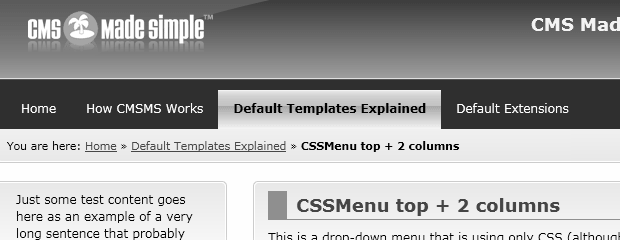
\includegraphics[width=0.9\textwidth, height=5cm]{cms_made_simple-gray}
\caption{\textlatin{CMS Made Simple CMS}}
\label{fig:made_simpl}
\end{figure}

\section{\textlatin{Concrete5}}
Το \textlatin{Concrete5} δίνει τη δυνατότητα στους \textlatin{developers} να δημιουργήσουν μια ιστοσελίδα κυριολεκτικά σε δευτερόλεπτα. Παρέχει ένα εύκολο περιβάλλον διαχείρησης περιεχομένου, καθοριζόμενου μέσω \textlatin{point and click}, το οποίο επιτρέπει και σε μη τεχνικούς χρήστες να το χειρίζονται και να μεταβάλλουν το περιεχόμενο.
\begin{figure}[H]
\centering
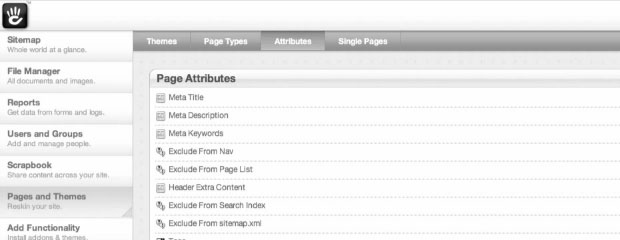
\includegraphics[width=0.9\textwidth, height=5cm]{Concrete5-gray}
\caption{\textlatin{Concrete5 CMS}}
\label{fig:concrete5}
\end{figure}

\section{\textlatin{Website Baker}}
Το \textlatin{Website Baker} επιτρέπει τη δημιουργία \textlatin{templates} ιστοσελίδων μέσα σε λίγα λεπτά. Το \textlatin{CMS} στηρίζεται πάνω σε \textlatin{(X)HTML, CSS} και \textlatin{jQuery}. Η επαύξηση των λειτουργιών του γίνεται με τη χρήση \textlatin{droplets}, τα οποία είναι κομμάτια κώδικα \textlatin{PHP} και τα οποία μπορούν να εισαχθούν σχεδόν οπουδήποτε στο \textlatin{CMS}.
\begin{figure}[H]
\centering
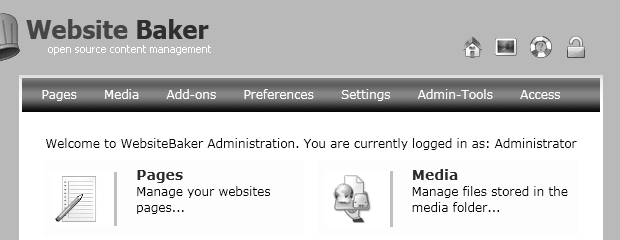
\includegraphics[width=0.9\textwidth, height=5cm]{websitebaker-gray}
\caption{\textlatin{Website Baker CMS}}
\label{fig:site_baker}
\end{figure}

\section{\textlatin{Umbraco}}
Το \textlatin{Umbraco} είναι ένα δωρεάν λογισμικό ανοιχτού κώδικα, το οποίο είναι βασισμένο πάνω στο \textlatin{Microsoft .NET Framework}. Είναι αρκετά εύχρηστο, απλό, κατανοητό και πλήρως επεκτάσιμο, με τη χρήση \textlatin{industry-standard} γλωσσών, όπως \textlatin{HTML, CSS, jQuery} και \textlatin{C\#}. Το \textlatin{Umbraco} είναι εξίσου ευέλικτο και δυνατό είτε χρησιμοποιείται από πεπειραμένους \textlatin{developers}, είτε από χρήστες που μόλις ξεκινούν να το χρησιμοποιούν.
\begin{figure}[H]
\centering
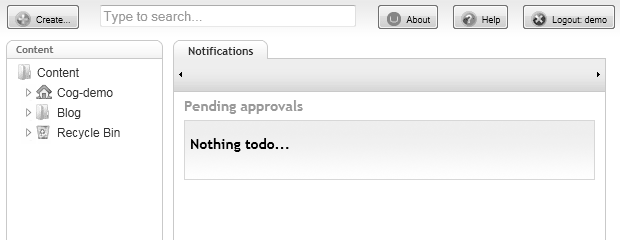
\includegraphics[width=0.9\textwidth, height=5cm]{umbraco-gray}
\caption{\textlatin{Umbraco CMS}}
\label{fig:umbraco}
\end{figure}

\section{\textlatin{Contao}}
Το \textlatin{Contao} έχει ένα αρκετά εύχρηστο και πλήρως πλοηγήσιμο περιβάλλον, το οποίο χρησιμοποιεί τεχνολογίες \textlatin{Ajax / Web 2.0} για βελτιστοποιημένη χρηστικότητα. Επίσης περιλαμβάνει πολλαπλά θέματα αλλά και διασυνδέσεις με πληθώρα γλωσσών \textlatin{backend}. Παρέχει, πέραν των άλλων, ισχυρό σύστημα διαχείρησης δικαιωμάτων \textlatin{versioning} κώδικα και διαχείριση αλλαγών (\textlatin{undo management}), εξελιγμένες επιλογές αναζήτησης και ταξινόμησης, καθώς και τη δυνατότητα εγκατάστασης ενημερώσεων εν θερμώ, τα οποία το καθιστούν ένα από τα πιο ολοκληρωμένα \textlatin{content management system (CMS)}. Το \textlatin{front end} του είναι 100\% βασισμένο στη χρήση \textlatin{templates}, και ο παραγώμενος κώδικας είναι πλήρως αναγνώσιμος και εναρμονισμένος με τις προδιαγραφές του \textlatin{W3C/WAI}.
\begin{figure}[H]
\centering
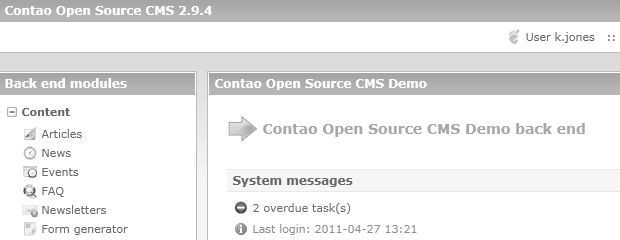
\includegraphics[width=0.9\textwidth, height=5cm]{Contao-gray}
\caption{\textlatin{Contao CMS}}
\label{fig:contao}
\end{figure}

\section{\textlatin{Plone CMS}}
Το \textlatin{Plone} είναι ένα \textlatin{CMS}, το οποίο είναι προσανατολισμένο κυρίως στη χρήση \textlatin{application oriented}, ενώ ένα συνηθισμένο \textlatin{CMS} είναι συνήθως προσανατολισμένο στη δημιουργία σελίδων. Εάν οι χρήστες ενός συστήματος θέλουν να προσθέσουν, διορθώσουν ή αφαιρέσουν περιεχόμενο, το οποίο προϋποθέτει διεργασίες ή περίπλοκους τύπους δεδομένων βασισμένους στη φυσική διάρθρωση ενός οργανισμού, τότε το \textlatin{Plone} είναι ίσως η καταλληλότερη επιλογή.
\begin{figure}[H]
\centering
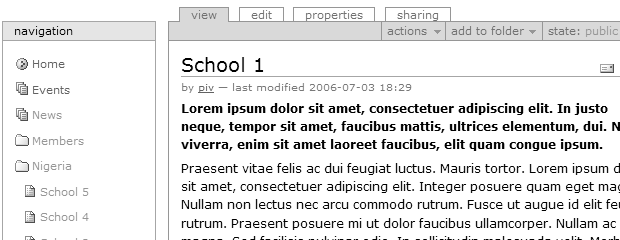
\includegraphics[width=0.9\textwidth, height=5cm]{plone_cms-gray}
\caption{\textlatin{Plone CMS}}
\label{fig:plone}
\end{figure}

\section{\textlatin{XOOPS}}
Το \textlatin{XOOPS} είναι ένα \textlatin{web application platform} το οποίο στηρίζεται στη γλώσσα \textlatin{PHP} και την ύπαρξη μιας βάσης δεδομένων \textlatin{MySQL}. Η αντικειμενοστραφής του σχεδίαση το κάνει ιδανικό εργαλείο για την ανάπτυξη ιστοσελίδων ποικίλου μεγέθους, \textlatin{corporate portals, weblogs} κ.α.
\begin{figure}[H]
\centering
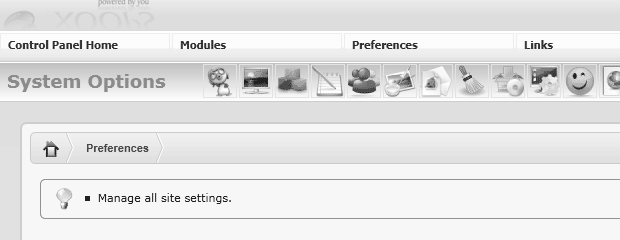
\includegraphics[width=0.9\textwidth, height=5cm]{xoops-gray}
\caption{\textlatin{XOOPS CMS}}
\label{fig:xoops}
\end{figure}

\section{\textlatin{MODX}}
Το \textlatin{MODx} παρέχει ένα ασφαλές περιβάλλον διαχείρησης, με το οποίο είναι δυνατό να δημιουργήσει κανείς μια ιστοσελίδα με ασφαλή τρόπο. Για παράδειγμα παρέχεται ένα σύστημα διαχωρισμού των χρηστών και διαχειριστών της ιστοσελίδας. Όσον αφορά τη διαχείριση περιεχομένου, παρέχεται η δυνατότητα κλωνοποίησης εγγράφων, δεδομένων ακόμα και ολόκληρων φακέλων σε απεριόριστο βάθος.
\begin{figure}[H]
\centering
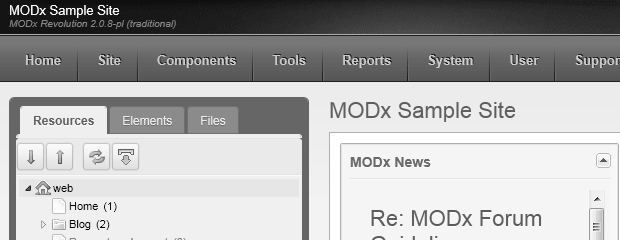
\includegraphics[width=0.9\textwidth, height=5cm]{modx-gray}
\caption{\textlatin{MODX CMS}}
\label{fig:modx}
\end{figure}

\section{\textlatin{Silverstripe}}
Το \textlatin{SilverStripe} είναι ένα αρκετά απλό \textlatin{CMS} ανοιχτού λογισμικού, το οποίο χρησιμοποιείται από πολλούς επαγγελματίες \textlatin{developers} για τη δημιουργία δυναμικού περιεχομένου. Το γεγονός ότι είναι πολύ εύχρηστο, το καθιστά ιδανική επιλογή και για μη τεχνικούς-χρήστες, οι οποίοι επιθυμούν να δημιουργήσουν εύκολα και γρήγορα έναν ιστότοπο.
\begin{figure}[H]
\centering
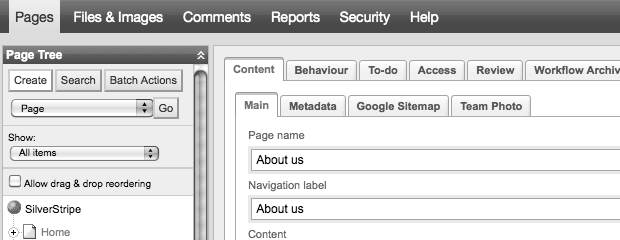
\includegraphics[width=0.9\textwidth, height=5cm]{silverstripe-gray}
\caption{\textlatin{Silverstripe CMS}}
\label{fig:silverstripe}
\end{figure}

\section{\textlatin{PyroCMS}}
Το \textlatin{PyroCMS} είναι αρκετά εύκολο, έχει καλή εμφάνιση και είναι εύκολο στη χρήση του. Εκτός αυτού, χρησιμοποιεί ένα σύστημα έξυπνου \textlatin{caching} για να αυξάνει την ταχύτητα απόκρισης. Είναι εύκολα επεκτάσιμο με αρθρώματα και πρόσθετα, ενώ το γεγονός ότι στηρίζεται στο \textlatin{CodeIgniter framework}, το καθιστά εύκολα τροποποιήσιμο όσον αφορά στην εμφάνιση του ιστοτόπου, με τη χρήση θεμάτων, τα οποία είναι απλός κώδικας \textlatin{HTML}.
\begin{figure}[H]
\centering
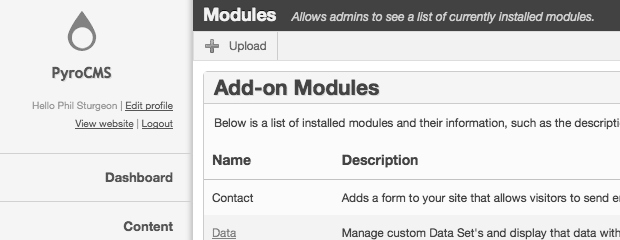
\includegraphics[width=0.9\textwidth, height=5cm]{pyrocms-gray}
\caption{\textlatin{PyroCMS CMS}}
\label{fig:pyrocms}
\end{figure}

\section{\textlatin{GetSimple CMS}}
Το \textlatin{GetSimple} είναι ένα ελαφρύ \textlatin{CMS} το οποίο στηρίζεται στη χρήση τεχνολογιών \textlatin{XML}. Παρόλο που είναι ελαφρύ, έχει όλες τις δυνατότητες που θα χρειαζόταν κάποιος για την δημιουργία και συντήρηση ενός ιστοτόπου μιας μικρής ή μεσαίας επιχείρησης.
\begin{figure}[H]
\centering
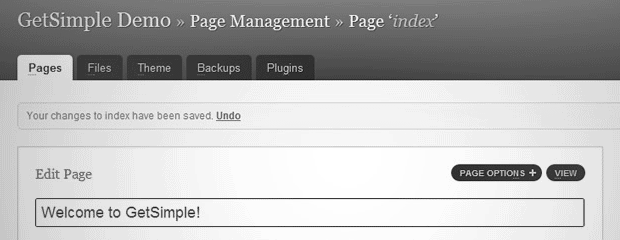
\includegraphics[width=0.9\textwidth, height=5cm]{getsimplecms-gray}
\caption{\textlatin{GetSimple CMS}}
\label{fig:get_simpl}
\end{figure}

\section{\textlatin{FuelCMS}}
Το \textlatin{FUEL CMS} είναι άλλο ένα \textlatin{CMS} το οποίο στηρίζεται στο \textlatin{CodeIgniter framework} και το οποίο είναι ελαφρύ, εξαιρετικά παραμετροποιήσιμο και επεκτάσιμο. Η χρήση του \textlatin{CodeIgniter framework} απαιτεί τη συγγραφή κώδικα και έτσι το \textlatin{FUEL CMS} απευθύνεται κυρίως σε επαγγελματίες \textlatin{developers}, χωρίς αυτό να σημαίνει ότι ένας απλός χρήστης δε μπορεί να το χρησιμοποιήσει, απλά για να ανεβάσει νέο περιεχόμενο.
\begin{figure}[H]
\centering
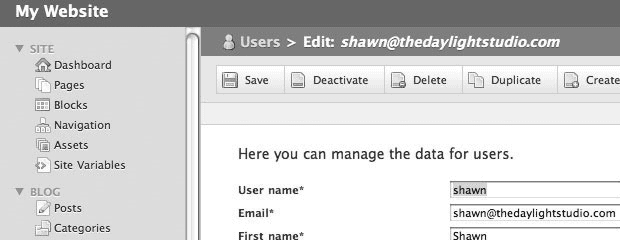
\includegraphics[width=0.9\textwidth, height=5cm]{fuelcms-gray}
\caption{\textlatin{FuelCMS CMS}}
\label{fig:fuelcms}
\end{figure}

\section{\textlatin{Drupal}}
To \textlatin{Drupal} είναι ένα ισχυρό και εξελιγμένο \textlatin{CMS framework} το οποίο στηρίζει την λειτουργία του στην γλώσσα \textlatin{php} και στην ύπαρξη μιας βάσης δεδομένων, όπως η \textlatin{MySQL}. To  \textlatin{Drupal} παρέχει ένα ευέλικτο περιβάλλον, το οποίο χρησιμοποιείται για τη διαχείριση ιστοτόπων διαφόρων τύπων και προφίλ. Το \textlatin{Drupal} μπορεί να χρησιμοποιηθεί για τη δημιουργία πλούσιων σε περιεχόμενο ιστοσελίδων με διαδραστικό περιεχόμενο, όπως φόρουμ, \textlatin{blogs} χρηστών και υπηρεσίες ανταλλαγής προσωπικών μηνυμάτων.

To \textlatin{Drupal} χρησιμοποιείται σε αρκετούς γνωστούς διαδικτυακούς τόπους, όπως για παράδειγμα το \textlatin{\url{http://www.weather.com}}. Καθώς βρίσκεται σε ενεργό κύκλο ανάπτυξης, αναβαθμίζεται αρκετά συχνά (σχεδόν κάθε 2 - 4 μήνες). Η εκτεταμένη κοινότητα χρηστών παρακολουθεί τα σχετικά συνέδρια, τα οποία λαμβάνουν χώρα κάθε 2 χρόνια σε Ευρώπη και Αμερική.

Η δύναμη του \textlatin{Drupal} βρίσκεται στην καλά οργανωμένη δομή του. Το \textlatin{Drupal} ξεκινά με ένα βασικό σύνολο αρχείων, το οποίο μπορεί να εμπλουτισθεί στη συνέχεια με διάφορα πρόσθετα, όπως θέματα ή αρθρώματα, που αυξάνουν τη λειτουργικότητά του. Ο αρχικός πυρήνας των αρχείων μπορεί να έχει ένα βασικό σετ από πρόσθετα ή θέματα, τα οποία μπορούν να τροποποιηθούν κατά βούληση.

Πέρα από τις παραπάνω παραμετροποιήσεις, υπάρχει διαθεσιμότητα σε σύνολα από πρόσθετα, τα οποία προορίζονται για συγκεκριμένη χρήση και συνήθως έρχονται με τη μορφή \textlatin{Drupal} διανομών. Διατίθενται για παράδειγμα διανομές για απλές εταιρικές ιστοσελίδες, για ενημερωτικού τύπου - πολυμεσικές ή ακόμα και διανομές γενικής χρήσης \textlatin{community-based}~\cite{opensource_cms_demos_and_information}.

\section{\textlatin{Joomla}}
Το \textlatin{Joomla} αναπτύσσεται ενεργά από το 2005 και χρησιμοποιείται σε πολύ γνωστές ιστοσελίδες όπως τις \textlatin{eBay, General Electric, Ikea} κ.α. Το \textlatin{Joomla} συγκριτικά με το \textlatin{Drupal}, το οποίο έχει περισσότερα πρόσθετα και θέματα, εμφανίζεται και αυτό αρκετά ενισχυμένο σε πλήθος πρόσθετων και επεκτάσεων. Εκτός αυτού, η βάση χρηστών και των δύο \textlatin{CMS} είναι αρκετά εκτεταμένη και έτσι είναι αρκετά εύκολη η εύρεση οδηγιών στο διαδίκτυο για αντιμετώπιση διαφόρων προβλημάτων.

Το \textlatin{Joomla} απευθύνεται κυρίως σε χρήστες μέσου επιπέδου γνώσεων~\cite{pixelmedia}. Διαθέτει εργαλεία για την συνεργατική ανάπτυξη ενός ιστοτόπου, αλλά και για κεντρικοποιημένη διαχείριση της διαδικασίας ανάπτυξης. Η διαδικασία εγκατάστασης δεν είναι ιδιαίτερα δύσκολη, αλλά η δημιουργία περιεχομένου δεν είναι τόσο εύκολη σε σχέση με το επόμενο προς εξέταση \textlatin{CMS}, το \textlatin{Wordpress}.

\section{\textlatin{Wordpress}}
Το \textlatin{Wordpress} δημιουργήθηκε αρχικά ως μια πλατφόρμα για τη δημιουργία και συντήρηση \textlatin{blogs}. Είναι μέχρι σήμερα, χωρίς αμφιβολία η ευκολότερη στη χρήση πλατφόρμα και ίσως η πιο δημοφιλής. Η ανάπτυξή της ξεκίνησε το 2003 και είναι ενεργή μέχρι σήμερα. Χρησιμοποιείται ήδη σε 60 εκατομμύρια περίπου ιστότοπους με ρυθμό αύξησης περίπου 100.000 νέους ιστότοπους ανά ημέρα.

Το \textlatin{Wordpress} είναι καλύτερο για την δημιουργία στατικού περιεχομένου. Αυτό δε σημαίνει όμως ότι δε μπορεί να χρησιμοποιηθεί και για δυναμικό ή περίπλοκο περιεχόμενο, καθώς η μεγάλη βάση χρηστών του έχει προσθέσει πλήθος λειτουργιών. Σήμερα η ανάπτυξή του καθοδηγείται ενεργά από την εταιρία \textlatin{Automattic}, με την απήχησή του να γίνεται όλο και μεγαλύτερη.

\section{Σύγκριση των πιο Δημοφιλών \textlatin{CMS}}
Στα προηγούμενα αναφέρθηκαν συνοπτικά τα πιο γνωστά \textlatin{CMS} ανοιχτού κώδικα. Στο παρόν αναλύονται τα τρία πιο δημοφιλή \textlatin{CMS} με τα πλεονεκτήματα και μειονεκτήματά τους και δίνεται ένας συνοπτικός πίνακας με τα πιο σημαντικά χαρακτηριστικά τους.

\subsection{\textlatin{WordPress} το πιο δημοφιλές \textlatin{CMS}}.
Παρά την ταπεινή του καταγωγή από το χώρο του \textlatin{bloging}, το \textlatin{WordPress} έχει επί της ουσίας κατακτήσει την αγορά των \textlatin{CMS}, με τα ποσοστά χρήσης του να αγγίζουν το 40\% των ιστότοπων που βασίζονται σε κάποιο \textlatin{CMS}.

Τα πλεονεκτήματά του περιλαμβάνουν:
\begin{itemize}
\item Εύκολη εγκατάσταση. Πολλές εταιρίες παροχής υπηρεσιών \textlatin{hosting} παρέχουν αυτοματοποιημένα εργαλεία εγκατάστασης και παραμετροποίησης ενός νέου ιστότοπου σε \textlatin{Wordpress}. Αυτό σημαίνει ότι οποιοσδήποτε μπορεί να έχει ένα νέο ιστότοπο, έτοιμο προς παραμετροποίηση μέσα σε 5 λεπτά.

\item Δυνατότητες Παραμετροποίησης. Το \textlatin{WordPress} έχει σημαντικά μεγαλύτερο αριθμό πρόσθετων, θεμάτων και επιλογών παραμετροποίησης από οποιοδήποτε άλλο \textlatin{CMS}. Εξαιτίας της μεγάλης του δημοφιλίας, όλο και περισσότεροι προγραμματιστές αναπτύσσουν εργαλεία, δωρεάν ή με ένα μικρό κόστος, για την παραμετροποίηση του \textlatin{WordPress}. Τα εργαλεία αυτά δίνουν τη δυνατότητα για τη δημιουργία ενός ιστοτόπου με εμφάνιση που παραπέμπει σε αντίστοιχα επαγγελματικά με ένα μικρό κόστος γύρω στα 100 Ευρώ.κόστος.

\item Δωρεάν. 
Free– WordPress is absolutely, no-strings-attached free to use. And building on the last point, there are easily tens of thousands of free plug-ins and themes available to choose from. This is perfect for most beginners putting together their first site because it keeps costs down.
Community Support – If you do experience issues or have questions about your new WordPress site, you can easily tap into the millions of people already using and supporting it. Their support forum includes helpful contributors that can answer any question you might have, within minutes, again – for free. Awesome, right?

Of course, WordPress isn’t perfect and does have it’s drawbacks.

Cheif among them: WordPress is an easy-to-use framework because it locks down the ability for most users to make significant visual edits (for their own good). So you can’t make a TON of structural website changes without the help of a designer and/or developer.

However, for a beginner, this is probably the most suitable platform to build a site.
  Drupal (More Robust & Complex)

Drupal is the third most popular content management system available today, used by sites both large and small.

It’s among the most powerful open sourced options available, which means it’s learning curve is also a bit steeper.

Here’s where Drupal excels:

    Technically Advanced – Drupal is the most technically advanced of these three content management systems. Good for technical people who like to get their hands dirty.
    Improved Performance – Drupal pages typically load more quickly, and have faster response times than those made with WordPress or Joomla. Part of the reason is because it’s less resource-intensive, requiring a less expensive server or hosting setup. (However like with all CMS, adding too many third party plugins can bog down performance.)
    Customizable – Drupal is easy to customize with many widely available plug-ins, themes and other configurable options to choose from. You can also edit the root files directly, perfect for those developers who need to make more significant changes.
    Free – You can download the Drupal software for free, and install it on your own hosting server. If you don’t which host to use, use this best web hosting chart.

Drupal is the most powerful content management system out of the box. But with that power comes some additional difficulties for the website owner.

Anyone considering Drupal should have at least a basic knowledge of HTML, PHP and other common web programming languages. You don’t need to be an expert necessarily, but being able to troubleshoot error messages and identify code problems will be a HUGE benefit.

If your website begins to gain traction, evolving beyond a simple business site or site, you’ll need to have (or hire) technical expertise to make sure it continues to run smoothly.

Which can be a bit of a problem, because it’s typically a little harder (and more expensive) to find someone with advanced knowledge of Drupal’s steep learning curve. Whereas it should be much easier and less expensive to find someone relatively tech-savvy to help you make basic WordPress updates.

Also, unlike WordPress.com, there is no option to have a website hosted by Drupal themselves. That means purchasing your own domain and hosting is required before getting started with a new Drupal site.
  Joomla (Somewhere Between WordPress & Drupal)

Joomla is the second most popular CMS. It’s like the compromise between WordPress and Drupal.

It’s powerful enough to run most websites without any problems, and it doesn’t require the same level of technical experience to run as Drupal either.

As the second most used CMS (behind WordPress), Joomla also has a lot of plug-ins and themes available to choose from (around 6000 or so) similar to both WordPress and Drupal. So customizing the look and feel of your site shouldn’t be problem.

Here are a few more reasons Joomla might be ideal for you:

    Social Networking – Joomla makes creating social networks of all three options. Social networks can be a powerful asset for many sites, and with Joomla, you can have one up and running extremely quickly and easily.
    Commerce Sites – Joomla also makes setting up an online store quick and painless. You can setup eCommerce shops with both Drupal and WordPress, but it tends to require more effort and special customizations.
    Not too Technical – Joomla has found the middle ground between the ease of managing a WordPress website and the power of a Drupal site. The good news is that most non-tech savvy people should be able to run a great Joomla site without needing any technical support.
    Help Portal – Joomla offers a great help portal for asking questions and getting technical support. It’s not fast or extensive as WordPress’ community-based support pages, but is definitely quicker (and cheaper) than Drupal’s technical support options.
    Free – Like both WordPress and Drupal, Joomla is another free option to use on your own web servers. However similar to Drupal, there is no option to have it hosted for free like WordPress offers.

Joomla users love that their websites can do or be almost anything, without sacrificing ease-of-use. Joomla has brilliantly combined the power and flexibility Drupal has to offer, while also retaining the intuitive, user-friendliness that WordPress excels at, making it a perfect middle ground in a crowded marketplace.
Making Your Choice

Και οι τρεις επιλογές είναι αρκετά καλές στην πλειονότητα των περιπτώσεων. Παρόλα αυτά υπάρχει πάντα μια πιθανότητα μια επιλογή να ταιριάζει καλύτερα σε ένα σενάριο, από ότι μια άλλη. Εάν κάποιος θέλει να ξεκινήσει έναν ιστότοπο σχετικά γρήγορα, τότε το \textlatin{Wordpress} είναι η καλύτερη λύση. Αν υπάρχει η πιθανότητα ο ιστότοπος κάποια στιγμή να μεγεθυνθεί μελλοντικά, με απαίτηση για εξελιγμένες δυνατότητες και χαρακτηριστικά, τότε το \textlatin{Drupal} είναι η καλύτερη επιλογή. Ανάμεσα στις δύο αυτές επιλογές βρίσκεται το \textlatin{Joomla}, το οποίο εμφανίζεται καλύτερη επιλογή για ιστότοπους κοινωνικής δικτύωσης ή μικρά ηλεκτρονικά καταστήματα.

Συνοψίζοντας μπορούμε να καταλήξουμε στα εξής αδρά συμπεράσματα:
\begin{itemize}
\item \textlatin{WordPress} – Η καλύτερη επιλογή για αρχάριους, λόγω της ευκολίας χρήσης του. Δουλεύει εξαιρετικά καλά για μικρούς έως μεσαίους ιστότοπους, \textlatin{blogs} και μικρά \textlatin{e-commerce} καταστήματα.
\item \textlatin{Joomla} – Είναι πολύ καλή επιλογή για ιστότοπους κοινωνικής δικτύωσης, αλλά απαιτεί μια βασική κατανόηση και κατοχή τεχνικών γνώσεων.
\item \textlatin{Drupal} – Είναι το πιο δύσκολο από τα τρία, αλλά επίσης και το πιο ισχυρό εργαλείο. Απαιτεί μια σχετική οικειότητα με γλώσσες όπως οι \textlatin{HTML, CSS and PHP}.
\end{itemize}

Στον παρακάτω πίνακα συγκρίνονται τα τρία παραπάνω \textlatin{CMS} με βάση τα διάφορα ετερογενή χαρακτηριστικά τους~\cite{comparison_tables}.

\selectlanguage{english}
\tiny
\begin{longtable}[H]{|| p{.3\linewidth} | p{.19\linewidth} | p{.19\linewidth} | p{.19\linewidth} ||}
\hline
\textbf{Atribute} & \textbf{Drupal} & \textbf{Joomla} & \textbf{WordPress} \\
\hline\hline \endhead
Website & drupal.org & joomla.org & wordpress.org \\
Latest version & 8.1.3 & 3.6 & 4.6.1 \\
Release date & 2016 Jun 15 & 2016 Aug 4 & 2016 Sep 7 \\
License & Open Source & Open Source & Open Source \\
Supported databases & MySQL, PostgreSQL & MySQL, PostgreSQL, SQL Server & MySQL \\
Platform & PHP & PHP & PHP \\
Security Captcha & No (Plugin Only) & No (Plugin Only) & No (Plugin Only) \\
Content Approval & Yes & Yes & Yes \\
Email Verification & Yes & Yes & Yes \\
Granular Privileges & Yes & Yes & Yes \\
Authentication methods & LDAP (plugin), NTLM (plugin), Custom & LDAP, Custom & LDAP (plugin), Custom \\
Session Management & Yes & Yes & No (Plugin Only) \\
SSL Compatible & Yes & Yes & Yes \\
Login History & Yes & Yes & No (Plugin Only) \\
Modifications History & Yes & No (Plugin Only) & No (Plugin Only) \\
Commercial Support & Yes & Yes & Yes \\
Developer Community & Yes & Yes & Yes \\
Public Forum & Yes & Yes & Yes \\
Plugin API & Yes & Yes & Yes \\
Drag \& Drop Content & No (Plugin Only) & Yes & Yes \\
Image Resizing & No (Plugin Only) & Yes & Yes \\
Multiple Upload & No (Plugin Only) & Yes & Yes \\
Spellchecker & No (Plugin Only) & No (Plugin Only) & Yes \\
Style Wizard & No (Limited) & No & No \\
Subscriptions & No (Plugin Only) & No (Plugin Only) & No (Plugin Only) \\
Template Language & Yes (Limited) & Yes & No \\
Undo & Yes (Limited) & No & Yes (Limited) \\
WYSIWYG Editor & No (Plugin Only) & Yes & Yes \\
Extensible User Profiles & Yes & Yes & No (Plugin Only) \\
Interface Localization & Yes & Ye & Yes \\
Performance \& Caching & Yes & Yes & No (Plugin Only) \\
Load Balancing & Yes (Limited) & Yes & Yes (Limited) \\
Database Replication & Yes (Limited) & Yes & No (Plugin Only) \\
Static Content Export & No & No & No (Plugin Only) \\
Multilingual Content & Yes & No (Plugin Only) & No (Plugin Only) \\
Multi-Site Deployment & Yes & No (Plugin Only) & Yes \\
RSS (Content Syndication) & Yes & Yes & Yes \\
Advertising Management & No (Plugin Only) & Yes & No \\
Content Scheduling & No (Plugin Only) & Yes & Yes (Limited) \\
Inline Administration & Yes & Yes & No (Plugin Only) \\
Package Deployment & No & No & No \\
Sub-sites / Roots & Yes & Yes & Yes \\
Themes / Templates & Yes & Yes & Yes \\
Web Statistics & Yes & Yes & No (Plugin Only) \\
Web-based Translation Management & Yes & No (Plugin Only) & Yes (Limited) \\
Workflow Engine & Yes (Limited) & No (Plugin Only) & No \\
FTP Support & Yes (Limited) & Yes & No (Plugin Only) \\
UTF-8 Support & Yes & Yes & Yes \\
WebDAV Support & No & No & No \\
XHTML Compliant & Yes & Yes & Yes \\
Blog & Yes & Yes & Yes \\
Chat & No (Plugin Only) & No (Plugin Only) & No (Plugin Only) \\
Classifieds & No (Plugin Only) & No (Plugin Only) & No (Plugin Only) \\
Contact Management & No (Plugin Only) & Yes & No (Plugin Only) \\
Forum (Discussion) & Yes & No (Plugin Only) & No (Plugin Only) \\
Document Management & Yes (Limited) & No (Plugin Only) & No \\
Events Management & No (Plugin Only) & No (Plugin Only) & No (Plugin Only) \\
FAQ Management & Yes & Yes & No (Plugin Only) \\
File Distribution & No (Plugin Only) & No (Plugin Only) & No (Plugin Only) \\
Graphs and Charts & No & No (Plugin Only) & No \\
Guestbook & No (Plugin Only) & No (Plugin Only) & No (Plugin Only) \\
Help Desk / Bug Reporting & No (Plugin Only) & No (Plugin Only) & No \\
Job Postings & No (Plugin Only) & No (Plugin Only) & No (Plugin Only) \\
Link Management & No (Plugin Only) & Yes & Yes \\
Mail Form & No (Plugin Only) & Yes & No (Plugin Only) \\
Matrix & No & No & No \\
My Page / Dashboard & No (Plugin Only) & Yes & Yes \\
Newsletter management & No (Plugin Only) & No (Plugin Only) & No (Plugin Only) \\
Photo Gallery & No (Plugin Only) & No (Plugin Only) & Yes \\
Project Tracking & No (Plugin Only) & No (Plugin Only) & No \\
Search Engine & Yes & Yes & Yes \\
Polls & Yes & Yes & No (Plugin Only) \\
Tests / Quizzes & No (Plugin Only) & No (Plugin Only) & No (Plugin Only) \\
Surveys & No (Plugin Only) & No (Plugin Only) & No (Plugin Only) \\
Time Tracking & No (Plugin Only) & No (Plugin Only) & No (Plugin Only) \\
WYSIWYG & No (Plugin Only) & Yes & Yes \\
User Contributions & Yes & Yes & Yes \\
Web Services Front End & Yes (Limited) & Yes & No (Plugin Only) \\
Wiki & No (Plugin Only) & No (Plugin Only) & No (Plugin Only) \\
Shopping Cart & No (Plugin Only) & No (Plugin Only) & No (Plugin Only) \\
SEO Metadata & Yes & Yes & Yes \\
SEO Friendly URLs & Yes & Yes & Yes \\
Site Map & No (Plugin Only) & No (Plugin Only) & No (Plugin Only) \\
\hline
\caption{\textgreek{Πίνακας Σύγκρισης} Open Source CMS}
\label{tab01}
\end{longtable}
\normalsize
\selectlanguage{greek}

\chapter{Ανάπτυξη Ιστοσελίδας Ηλεκτρονικών Δημοπρασιών}\label{ch3}
Για την ανάπτυξη της ιστοσελίδας της εργασίας χρησιμοποιήθηκε πλήθος εργαλείων, τα οποία στην πλειονότητά τους βρίσκονται διαθέσιμα δωρεάν στο Διαδίκτυο (\textlatin{Open Source Software}). Στα επόμενα γίνεται μια σύντομη αναφορά στα εργαλεία που χρησιμοποιήθηκαν και στη διαδικασία της ανάπτυξης.

\section{\textlatin{\textlatin{Vagrant (Open Source VM Provissioner)}}}\label{vagrant}
Το \textlatin{Vagrant} είναι ένα εργαλείο δημιουργίας και διαχείρησης εικονικών μηχανών με τη χρήση μιας εξαιρετικά απλοποιημένης διαδικασίας~\cite{vagrant_by_hashicorp}. Το εργαλείο αυτό δίνει έμφαση στην αυτοματοποιημένη διαχείριση των εικονικών μηχανών και μειώνει σημαντικά το χρόνο δημιουργίας και παραμετροποίησης ενός \textlatin{development server}.

Είναι γραμμένο στη γλώσσα προγραμματισμού \textlatin{Ruby} και αποτελεί έναν ενιαίο τρόπο επικοινωνίας με δίάφορους \textlatin{providers} εικονικών μηχανών (όπως \textlatin{VirtualBox, VMware, AWS} κ.α.). Με τον τρόπο αυτό είναι δυνατή η δημιουργία εικονικών μηχανών με τις επιθυμητές παραμέτρους στον μικρότερο δυνατό χρόνο. Παράλληλα, για την εγκατάσταση πακέτων λογισμικού αλλά και παραμετροποίηση σε επίπεδο λειτουργικού συστήματος (ΛΣ), είναι δυνατή η συνεργασία με ευρέως διαδεδομένα \textlatin{provisioning tools}, όπως \textlatin{Chef, Puppet, Ansible} ακόμα και με απλά \textlatin{shell scripts}.

Το μεγαλύτερο ίσως πλεονέκτημα του υπόψη εργαλείου είναι η δυνατότητα παροχής στους προγραμματιστές ενός ενιαίου περιβάλλοντος, το οποίο είναι σταθερό και όσο κοντά γίνεται στο παραγωγικό εξυπηρετητή. Επίσης επειδή η παραμετροποίηση γίνεται με αυτόματο τρόπο, αφαιρείται από τους προγραμματιστές το βάρος της δημιουργίας, συντήρησης και αποσφαλμάτωσης του περιβάλλοντος ανάπτυξης.

Η αρχή λειτουργίας του \textlatin{Vagrant} στηρίζεται στην ύπαρξη μιας εικονικής μηχανής στελέχους (\textlatin{template/vagrant box}), η οποία είναι διαθέσιμη από τα επίσημα αποθετήρια \textlatin{\url{https://vagrantcloud.com/boxes/search}} είτε μπορεί να είναι δική μας. Κατόπιν μέσω μιας διαδικασίας κλωνοποίησης και εφαρμογής παραμέτρων, εντελώς διαφανούς για το χρήστη, αποδίδεται η εικονική μηχανή.

Όλα τα παραπάνω γίνονται με την εκτέλεση της εντολής \textlatin{\texttt{vagrant}} ακολουθούμενης από το αντίστοιχο \textlatin{switch}. Για παράδειγμα, η παρακάτω ακολουθία εντολών κατεβάζει μια εικονική μηχανή \textlatin{ubuntu 64bit} από το επίσημο αποθετήριο και την θέτει σε λειτουργία με τη βοήθεια του \textlatin{VirtualBox}.
\selectlanguage{english}
\begin{Verbatim}
  $ vagrant box add ubuntu/xenial64
  $ vagrant init
  $ vagrant up --provider=virtualbox
\end{Verbatim}
\selectlanguage{greek}

Για τη φιλοξενία του ιστοτόπου της εργασίας χρησιμοποιήθηκε μια μηχανή \textlatin{centos7 64bit} από το επίσημο αποθετήριο. Επειδή η ανάπτυξη έγινε σε \textlatin{Fedora Linux}, χρησιμοποιήθηκε ως \textlatin{Virtualization provider} το παρεχόμενο από το ίδιο το λειτουργικό \textlatin{KVM / libvirt}. Στην συνέχεια με τη χρήση \textlatin{shell provissioner} έγινε η εγκατάσταση και παραμετροποίηση της βάσης δεδομένων (\textlatin{mariadb}) και του \textlatin{webserver (apache 2.4, php 5.4)}. Με τη χρήση του ίδιου \textlatin{provissioner} συγχρονίστηκε ο κώδικας και τέθηκαν τα σωστά \textlatin{filesystem permissions}.
Όλα τα παραπάνω ορίζονται στο αρχείο \textlatin{\texttt{Vagrantfile}} το οποίο παρατίθεται στο Παράρτημα~\ref{AppA}.

\section{Εγκατάσταση ιστοτόπου \textlatin{Drupal} Βήμα - Βήμα}\label{manual_setup}

\section{\textlatin{Ansible (Open Source Automation Provider)}}\label{ansible}
Ansible is software that automates software provisioning, configuration management, and application deployment.~\cite{geerling_2015}

Michael DeHaan, the author of the provisioning server application Cobbler and co-author of the Func framework for remote administration, developed the platform. It is included as part of the Fedora distribution of Linux, owned by Red Hat Inc., and is also available for Red Hat Enterprise Linux, CentOS, Scientific Linux and Oracle Linux via Extra Packages for Enterprise Linux (EPEL) as well as for other operating systems.[4]

Ansible, Inc. (originally AnsibleWorks, Inc.) was the company set up to commercially support and sponsor Ansible.[5][6] Red Hat acquired Ansible in October 2015.[7][8]

The name "Ansible" references a fictional instantaneous hyperspace communication system (as featured in Orson Scott Card's Ender's Game (1985),[9][10] and originally conceived by Ursula K. Le Guin for her novel Rocannon's World (1966)).

To orchestrate nodes, Ansible deploys modules to nodes over SSH. Modules are temporarily stored in the nodes and communicate with the controlling machine through a JSON protocol over the standard output.[13] When Ansible is not managing nodes, it does not consume resources because no daemons or programs are executing for Ansible in the background


\section{Συμπεράσματα}
Στο παρόν, παρουσιάστηκε η διαδικασία ανάπτυξης καθώς και η λειτουργικότητα μιας ιστοσελίδας ηλεκτρονικών δημοπρασιών. Έγινε αναφορά σε βασικές έννοιες του ηλεκτρονικού εμπορίου και των ηλεκτρονικών δημοπρασιών. Στη συνέχεια περιγράφηκαν τα εργαλεία τα οποία χρησιμοποιήθηκαν για την ανάπτυξη του ιστοτόπου της εργασίας και ο τρόπος με τον οποίο αυτοματοποιήθηκαν και συνδυάστηκαν για την παραγωγή του τελικού αποτελέσματος, μετά και τη διαδικασία αποσφαλμάτωσης. Τέλος παρουσιάστηκαν οι βασικές λειτουργίες της σελίδας με συνοπτικό τρόπο και τη βοήθεια ανάλογων \textlatin{screenshots}.

Η ιστοσελίδα της εργασίας παρέχει πλήρη λειτουργικότητα διεξαγωγής των δημοπρασιών, με αυτόματη ανανέωση της σελίδας και ενημέρωση των χρηστών για την πορεία της διαδικασίας. Εκτός αυτού, με τη διάκριση των ρόλων των χρηστών και την ασφαλή αυθεντικοποίηση μέσω φορμών εισαγωγής στοιχείων, παρέχεται η απαιτούμενη διασφάλιση της διαδικασίας. Λειτουργικότητες που δεν ενσωματώθηκαν στην εργασία, όπως πληρωμές με τραπεζικές κάρτες, \textlatin{paypal} κ.α παραλήφθηκαν για λόγους κόστους, όπως αναλύθηκε στο~\ref{phpprobid}.


\begin{appendices}
\chapter{Αρχείο Ρύθμισης Εικονικής Μηχανής \textlatin{Vagrantfile}}\label{AppA}
\selectlanguage{english}
\inputminted[linenos, fontsize=\scriptsize, breaklines, baselinestretch=1]{ruby}{sources/Vagrantfile}
\selectlanguage{greek}
\end{appendices}

\appendix

\bibliographystyle{babplain}
\bibliography{gnu-cms}

\end{document}